\chapter{Security and Efficiency}
\label{chap:4}

The role of the prover is to convince the verifier about the valid execution of a specified arithmetic circuit by showing that conditions form \Cref{sec:checks} are satisfied. This is done by constructing specific polynomials and proving their evaluation at uniformly randomly selected points using the KZG polynomial commitment scheme. It might not be directly clear from the diagram \Cref{fig:full-diagram}, but the whole protocol is basically a batched KZG for polynomials that prove valid execution of the circuit.

\begin{figure}
    \centering
    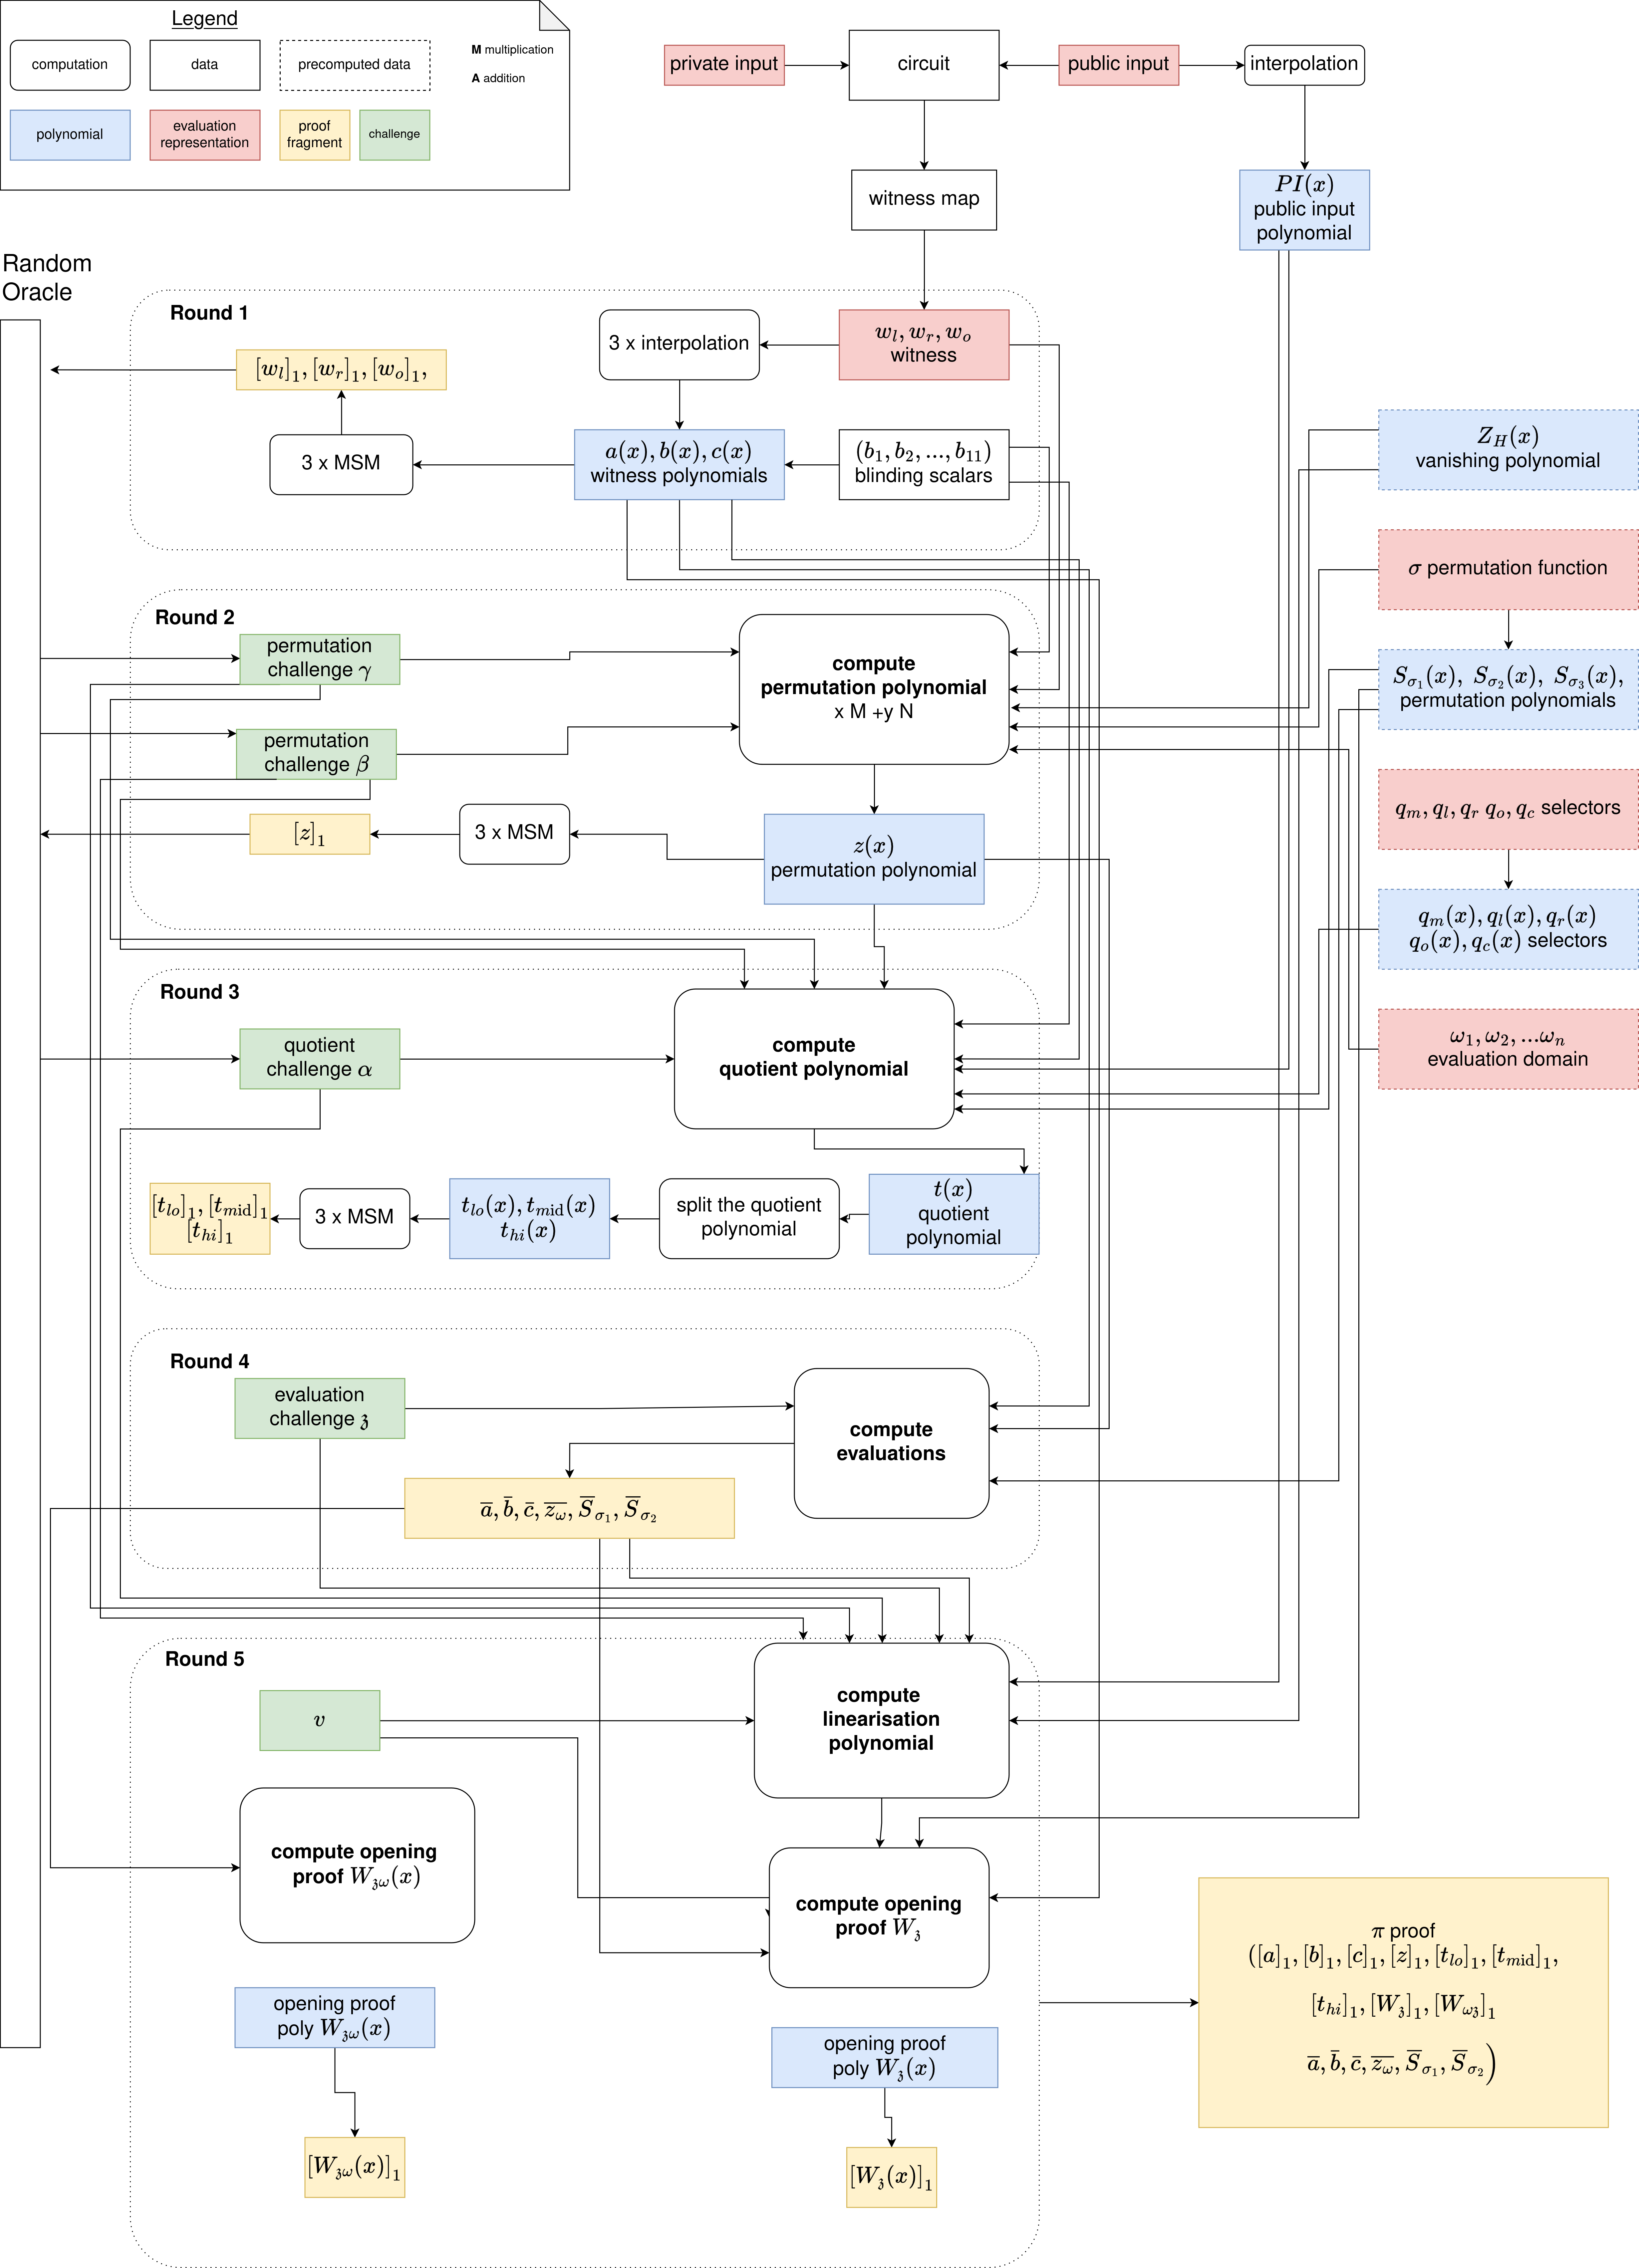
\includegraphics[width=1\linewidth]{round-figures/prover-algorithm.drawio.png}
    \caption{Diagram of prover algorithm}
    \label{fig:full-diagram}
\end{figure}

Degree bound on the polynomials constructed by the prover:
\begin{itemize}
    \item Wire polynomials $deg(a(x)) = deg(b(x)) = deg(c(x)) = n+1$ determined the multiplication of blinding polynomial of degree 1 and the vanishing polynomial of degree $n$.
    \item Permutation polynomial $deg(z(x)) = n+2$ determined by multiplication of blinding polynomial of degree 2 and vanishing polynomial of degree $n$
    \item Quotient polynomial $deg(t(x)) 3n+5$ described in the round 3 \Cref{sec:polynomial-splitting}
    \item Split quotient polynomials $deg(t_{lo}(x)) = deg(t_{mid}(x)) = n, deg(t_{hi}(x)) = n+5$ quotient polynomial is split into 3 smaller polynomials
    \item Linearisation polynomial $deg(r(x)) = n+5$ as described in round 4 \Cref{chap:round4} the linearisation polynomial cannot contain polynomial multiplication. Therefore, the degree is determined by the polynomial of the highest degree, which is $t_{hi}(x)$
    \item Opening proof polynomial $deg(W_{\challenge}(x)) = n+4$ degree is determined by $t(x)$ and consequently divided by $(x - \challenge)$
    \item Opening proof permutation polynomial $deg(W_{\challenge\omega}(x)) = n+1$ degree is determined by $z(x)$ and divided by $(x - \challenge\omega)$
\end{itemize}

\section{Advantages and limitations}

The plonk protocol can run for a general circuit of some size that is bounded by the $KZG$ setup. The setup, in the form of common preprocessed input, is updatable, and the trusted KZG setup can be reused for any circuit of a given size bound. Moreover, the size of the proof is constant. 

A downside of the protocol is the requirement for a trusted setup. As stated in the article \cite{pipeMSM}, the calculation of the commitments seems to be a major bottleneck of $\plonk$ and other SNARK protocols. Another major bottleneck is FFT. There is a lot of effort to make the prover algorithm more effective. Possible ways for the protocol optimization are mentioned in the \Cref{optimization-possibilities}. 



\section{Properties of the protocol}

\begin{theorem}
    \label{main-theorem}
    The $\plonk$ protocol is a succinct, non-interactive, complete, knowledge-sound, and zero-knowledge.
\end{theorem}

\paragraph{Succinctness:} The proof $\pi$ consists of 9 commitments and 6 openings, so for an arbitrarily large circuit, the proof size remains constant. The verification algorithm must perform sanity checks, evaluate 3 public polynomials, calculate 3 additional commitments, and perform a single batched KZG verification procedure. The number of operations does not change with respect to the size of the circuit, so we can conclude that the protocol is succinct.

\paragraph{Non-Interactivity:} Non-interactivity is achieved by the Fiat-Shamir heuristic, where the prover can effectively generate challenges by accessing a random oracle $\mathcal{H}$. We will not show the correctness of the application of this heuristic.

\paragraph{Completeness:} Correctness of $\plonk$ is dependant on many building blocks. Correctness of the checks for the arithmetic circuit was established by \Cref{input-correctness-soundness}, \Cref{output-correctness-soundness}, \Cref{gate-correctness-soundness}, \Cref{permutation-correctness-soundness}, and we also showed the correctness of the KZG polynomial commitment scheme \Cref{kzg-correctnes}.

\paragraph{Knowledge Soundness:} We showed the soundness of each of the checks for the arithmetic circuit \Cref{input-correctness-soundness}, \Cref{output-correctness-soundness}, \Cref{gate-correctness-soundness}, \Cref{permutation-correctness-soundness}. We did not show the soundness of KZG but referred to \cite{ProofArgsAndZk}.

\paragraph{Zero-Knowledge:} Since the proof contains only commitments and polynomial opening, it is sufficient to show that masking polynomial makes the KZG polynomial commitment scheme zero-knowledge, which was proven in \Cref{theorem:blinding}.

With respect to the above discussion, we can conclude the \Cref{main-theorem} is proven. 

